% ====================
\chapter{Motion Planning}
% ====================
% --------------------
\section{Introduction to Motion Planning}
% --------------------
An in-depth introduction can be found in Chapter 1.3 of Lavalle
\cite{lavalle2006planning}.
% \begin{itemize}
% \item State
% \item Time
% \item Actions
% \item Initial and Goal States
% \item Feasibility and Optimality Criterion
% \item A Plan
% \end{itemize}

% --------------------
\subsection{Simple Motion Planning}
% --------------------
The simplest motion planning problems assume knowledge of a global map, a fixed
known goal state and a fixed known initial state. The problem is to determine a
feasible path from the initial state to the goal state. An optimality criterion
may also be applied to choose the best path if multiple feasible ones are found.

Notably, two important concepts are ignored in determining the path:
differential constraints of the system and the use of feedback. Differential
constraints refer to how states transition to other states, and is inherent in
real-world systems, eg. a system's dynamics. For example, a car can easily move
fowards and backwards, but cannot immediately move side to side, which may be
assumed when determining a path. Feedback refers to the technique of refining
further actions based on newly sensed data. In simulations feedback may not be
necessary, but in real-world systems, errors in sensing and modeling build up
over time without it.

In this simple case, the solution involves a generated path that is followed in
an open-loop manner, or if subject to real-world constraints (see
\autoref{fig:lavalle2006planning119}), the generated path is smoothed to obey
the system's dynamics and feedback is used to closely follow the path. "Notably
this approach is highly decoupled as feedback and dynamics are neglected in
constructing the original path" \cite{lavalle2006planning}. The smooth path may
now obey the robot's dynamics, but may no longer be feasible. Feedback is used
as an inefficient afterthought to stay on a track that itself may not be
feasible or optimal.

\begin{figure}
\centering
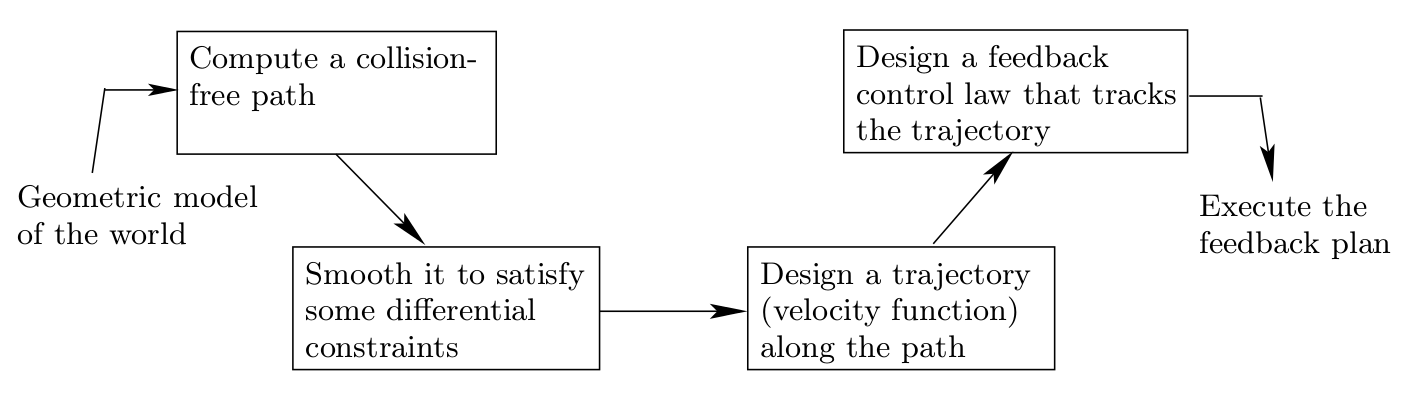
\includegraphics[width=3in]{figures/lavalle2006planning119.png}
\caption{From \cite{lavalle2006planning}. A refinement approach that has been
used for decades in robotics. Note the initial path is computed without
consideration of differential constraints or the use of feedback}
\label{fig:lavalle2006planning119}
\end{figure}

Even in this simple case, obtaining an optimal or even feasible path is not
straightforward if the state space is large. A* search for trivially sized state
spaces and sampling-based techniques such as RRTs (RRT* for optimality) and PRMs
have proven to be the methods of choice (citation?), though it is still an
ongoing field of interest (cite 2015 RRT/PRM papers).

The ROS Navigaiton Stack
(\url{http://www.dis.uniroma1.it/~nardi/Didattica/CAI/matdid/robot-programming-ROS-introduction-to-navigation.pdf})
is an example of this.
% --------------------
\subsection{Feedback Motion Planning}
% --------------------
Incorporating feedback directly when generating a path is a secondary option. 
For a full description of feedback motion planning, see Chapter 8 of Lavalle
\cite{lavalle2006planning}.
In the back-in parking problem, the trajectory to the goal state is assumed
visible, and hence generating a vector field may be suitable. A reliable model
and odometry data, however, varies from wheelchair to wheelchair, and so the
solution must be robust to model inaccuracies.

Two approaches can be taken: One, a target parking spot can be determined from
the initial position of the wheelchair, and the initial point cloud can be used
as a local map. The task is then to simultaneously localize the wheelchair's
position in the initial map while following a trajectory towards the parking
spot. This is visualized in \autoref{fig:determinedrive2}.
 
\begin{figure} % --------------------------------------
\centering
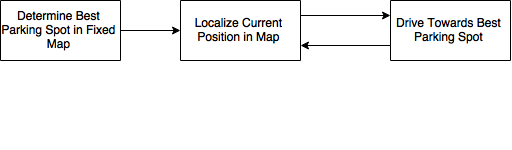
\includegraphics[width=3in]{figures/determinedrive2.png}
\caption{Feedback loop with a fixed goal state and map}
\label{fig:determinedrive2}
\end{figure}   % --------------------------------------

A second approach is to instead continuously update the initial map with new
sensor data, in effect performing SLAM on a constrained trajectory. The goal
state can then also be continously updated as new map information is ingested,
and the trajectory of the wheelchair will be updated based on this.
\autoref{fig:determinedrive1} illustrates this.
 
\begin{figure} % --------------------------------------
\centering
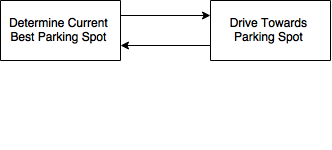
\includegraphics[width=3in]{figures/determinedrive1.png}
\caption{Feedback loop}
\label{fig:determinedrive1}
\end{figure}   % --------------------------------------

% ====================
\section{Related Work}
\label{sec:backinginlitreview}
% ====================
One way is to have a fixed, open-loop trajectory. This method is very old and
has been done for cars.

\cite{sermeno2006vision} uses vision-based PID control (page 17)

Angus's paper using PID

\subsection{Localization}
Talebifard \cite{talebifard2014risk} creates an egocentric map to avoid
localization.

\subsection{Real-time Motion Planning}

From \cite{hauser2013recognition}:
Sampling-based motion planners such as Probabilistic Roadmaps (PRMs) and
Rapidly-Exploring Random Trees (RRTs) are effective at planning collision-free
motion for high-dimensional robot systems ( LaValle 2006), and have also been
successfully applied to hard real-time planing for 2D helicopters ( Frazzoli et
al. 2002) and ground vehicles ( Petti and Fraichard 2005). Recently they have
been applied to teleoperation interfaces for robot manipulator arms ( Hauser
2011). But these works have traditionally focused on finding feasible paths
rather than optimal ones.  Sampling-based approaches have been recently
developed for the optimal motion planning problem ( Karaman and Frazzoli 2010),
but they have not yet been applied to time- varying cost functions and moreover
converge too slowly for real-time use. An alternative approach is numerical
opti- mization over a trajectory parameterization ( Bobrow et al.  2001).
Optimization approaches can achieve optimality with a fast convergence rate,
albeit only locally. Our hybrid plan- ner combines the strength of
sampling-based and numeri- cal approaches and is designed specifically to
produce high- quality paths quickly for a broad class of cost functions.

% ====================
\section{Implementation Details}
% ====================

% ====================
\section{Experimental Results}
% ====================

% 
% % --------------------
% \section{Practical Options}
% % --------------------
% 
% \begin{figure}
% \centering
% 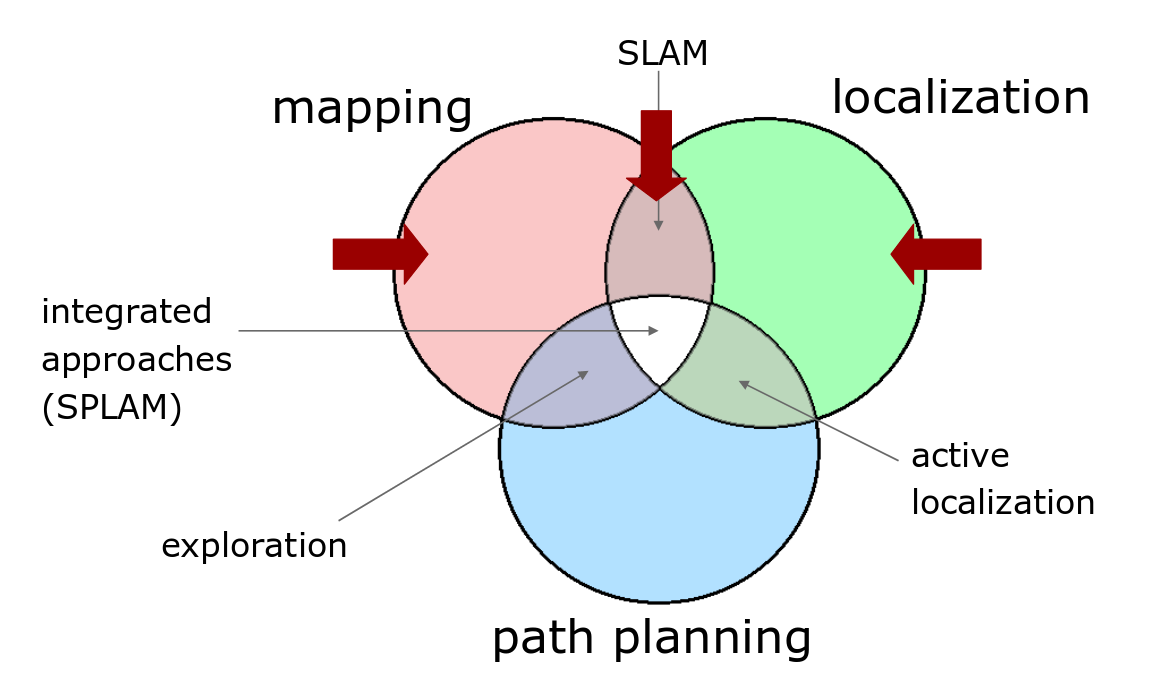
\includegraphics[width=3in]{figures/mappinglocalizationpathplanningvenndiagram.png}
% \caption{Venn Diagram of Localization, Mapping and Path Planning}
% \label{fig:mappinglocalizationpathplanningvenndiagram}
% \end{figure}
